\subsection{Editors}\label{sec:editors}

This section will describe the most relevant \acrfullpl{IDE} for \acrlong{emf} and the \gls{cloud}.

\subsubsection{Visual Studio Code}\label{sec:vscode}

\paragraph*{What it is}
Visual Studio Code (\gls{VSCode}) is a text editor and \acrfull{IDE} created by
Microsoft. The VSCode editor is based on the \gls{open source}\footnote{Source for VSCode is available at \href{https://github.com/microsoft/vscode}{https://github.com/microsoft/vscode}} software (OSS) called \emph{VS Code Project}.~\cite{helmingEclipseTheiaIDE2019} 
The VSCode editor has Microsoft-specific customizations, which makes it slightly different from the OSS project.~\cite{MicrosoftVscode2020} (This is analogous to the relationship between the \gls{open source} Chromium and the proprietary Google Chrome.)

\begin{figure}[htbp]
  \centering
  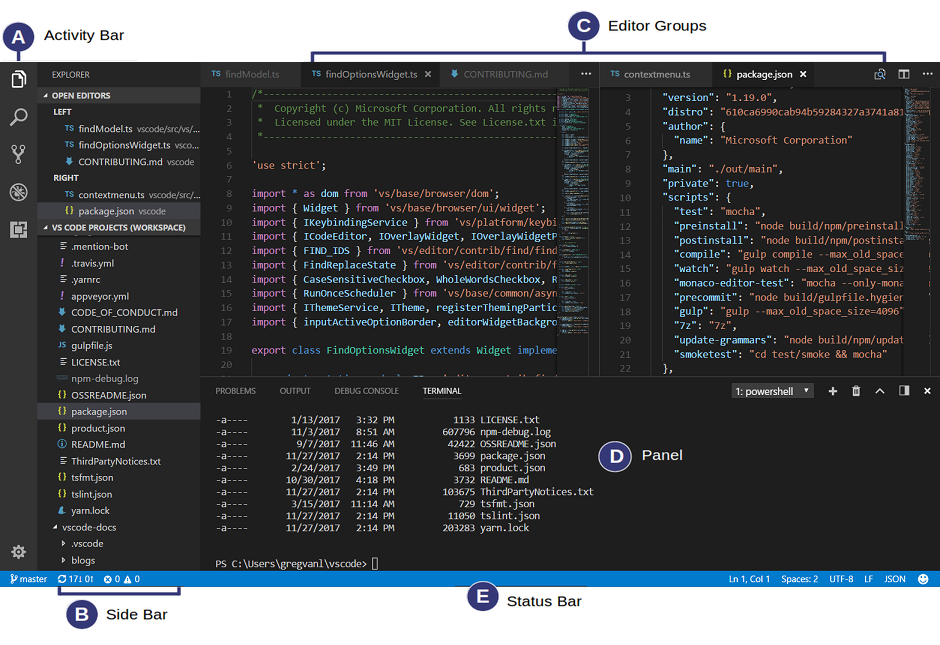
\includegraphics[width=\textwidth]{figures/vscode-ui}
  \caption[Visual Studio Code User Interface]{The user interface of Visual Studio Code, with annotations for the different components (\emph{A-E}).\cite{microsoftVisualStudioCode2020}}\label{fig:vscode-ui}
\end{figure}

\paragraph*{Intended use} Primarily an editor for textual programming languages.
VSCode has no support for diagrams or binary file viewers (like 3D models) out of the box (except pictures like \texttt{png} etc.). By default, it supports \texttt{Javascript}, \texttt{Typescript} and \texttt{Markdown}; common technologies related to web development.
VSCode can be extended to support other languages and editors, see \cref{chap:vscode-extension}.

% What does it do?
% Who made it?
% Architecture

\paragraph*{Architecture}
VSCode runs as a desktop application, and uses Electron and javascript for its runtime.
The architecture is centered on a \emph{core} which loads \emph{extensions}.
The core is shown in \cref{fig:vscode-layers-architecture}, and is split internally into \emph{layers} with different responsibilies.
Each layer is again organized based on the target runtime, like \emph{browser} or \emph{\gls{Electron}}, as seen in \cref{fig:vscode-component-architecture}.
The actual text editor in \gls{VSCode} is called \emph{Monaco}, and is available as a standalone package.~\cite{benjaminpaseroSourceCodeOrganization2020}


\begin{figure}[htbp]  % order of priority: h here, t top, b bottom, p page
  \centering %TODO: Fix the bad mermaid diagram layout
  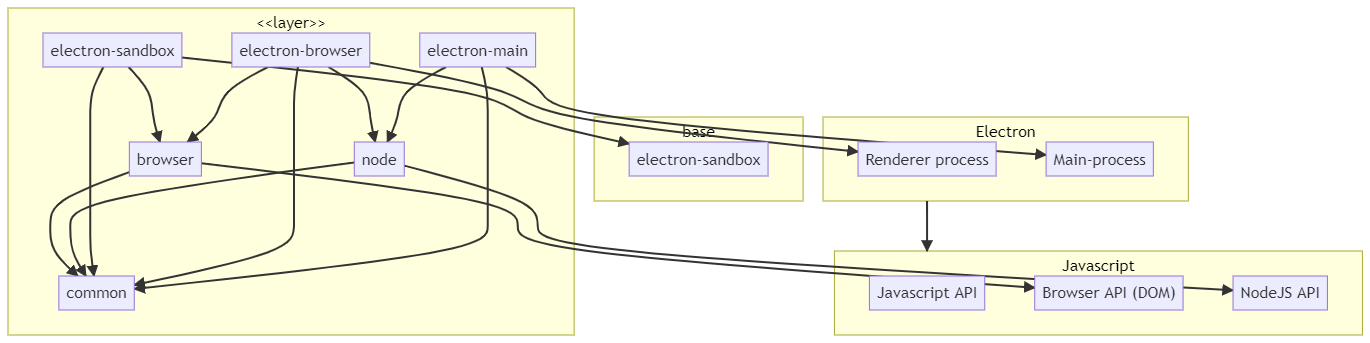
\includegraphics[width=\textwidth]{figures/vscode-component-architecture}
  \caption[VSCode component Architecture]{The internal architecture of each component in VSCode. The \texttt{<<layer>>} label represents each of the layers in \cref{fig:vscode-layers-architecture}, like \emph{base} or \emph{platform}. Every layer is organized by runtime dependencies.~\cite{benjaminpaseroSourceCodeOrganization2020}}\label{fig:vscode-component-architecture}
\end{figure}

\begin{figure}[htbp]
  \centering
  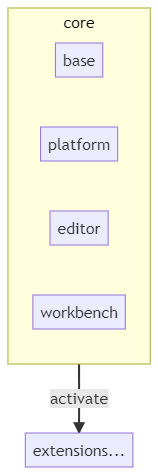
\includegraphics[width=2cm]{figures/vscode-layers-architecture}
  \caption[VSCode Layers]{The internal layers which the VSCode \texttt{core} is separated into.~\cite{benjaminpaseroSourceCodeOrganization2020}}\label{fig:vscode-layers-architecture}
\end{figure}



\subsubsection{Theia}\label{sec:theia}

\paragraph*{What it is}
\Gls{Theia} is an editor like \gls{VSCode}, but designed from the start to work in web browsers.
A screenshot is shown in \cref{fig:theia-user-interface}; notice how it is almost identical to \gls{VSCode}.
The project was originally started by TypeFox, and then donated to the Eclipse Foundation.
It is free and fully \gls{open source}\footnote{Source for Theia is available at \href{https://github.com/eclipse-theia/theia/}{https://github.com/eclipse-theia/theia/}}.
\Gls{Theia} is based on some of the same components as \gls{VSCode}, and uses Monaco as well.
The main uses of Theia now is as an editor for workspace software like \gls{Che} and \gls{Gitpod}.
Theia supports VSCode extensions, but not all of the \acrshortpl{API} in VSCode are implemented yet\footnote{A table of \acrshort{API} support is provided at \href{https://che-incubator.github.io/vscode-theia-comparator/status.html}{https://che-incubator.github.io/vscode-theia-comparator/status.html}.}.

\begin{figure}[htbp]
  \centering
  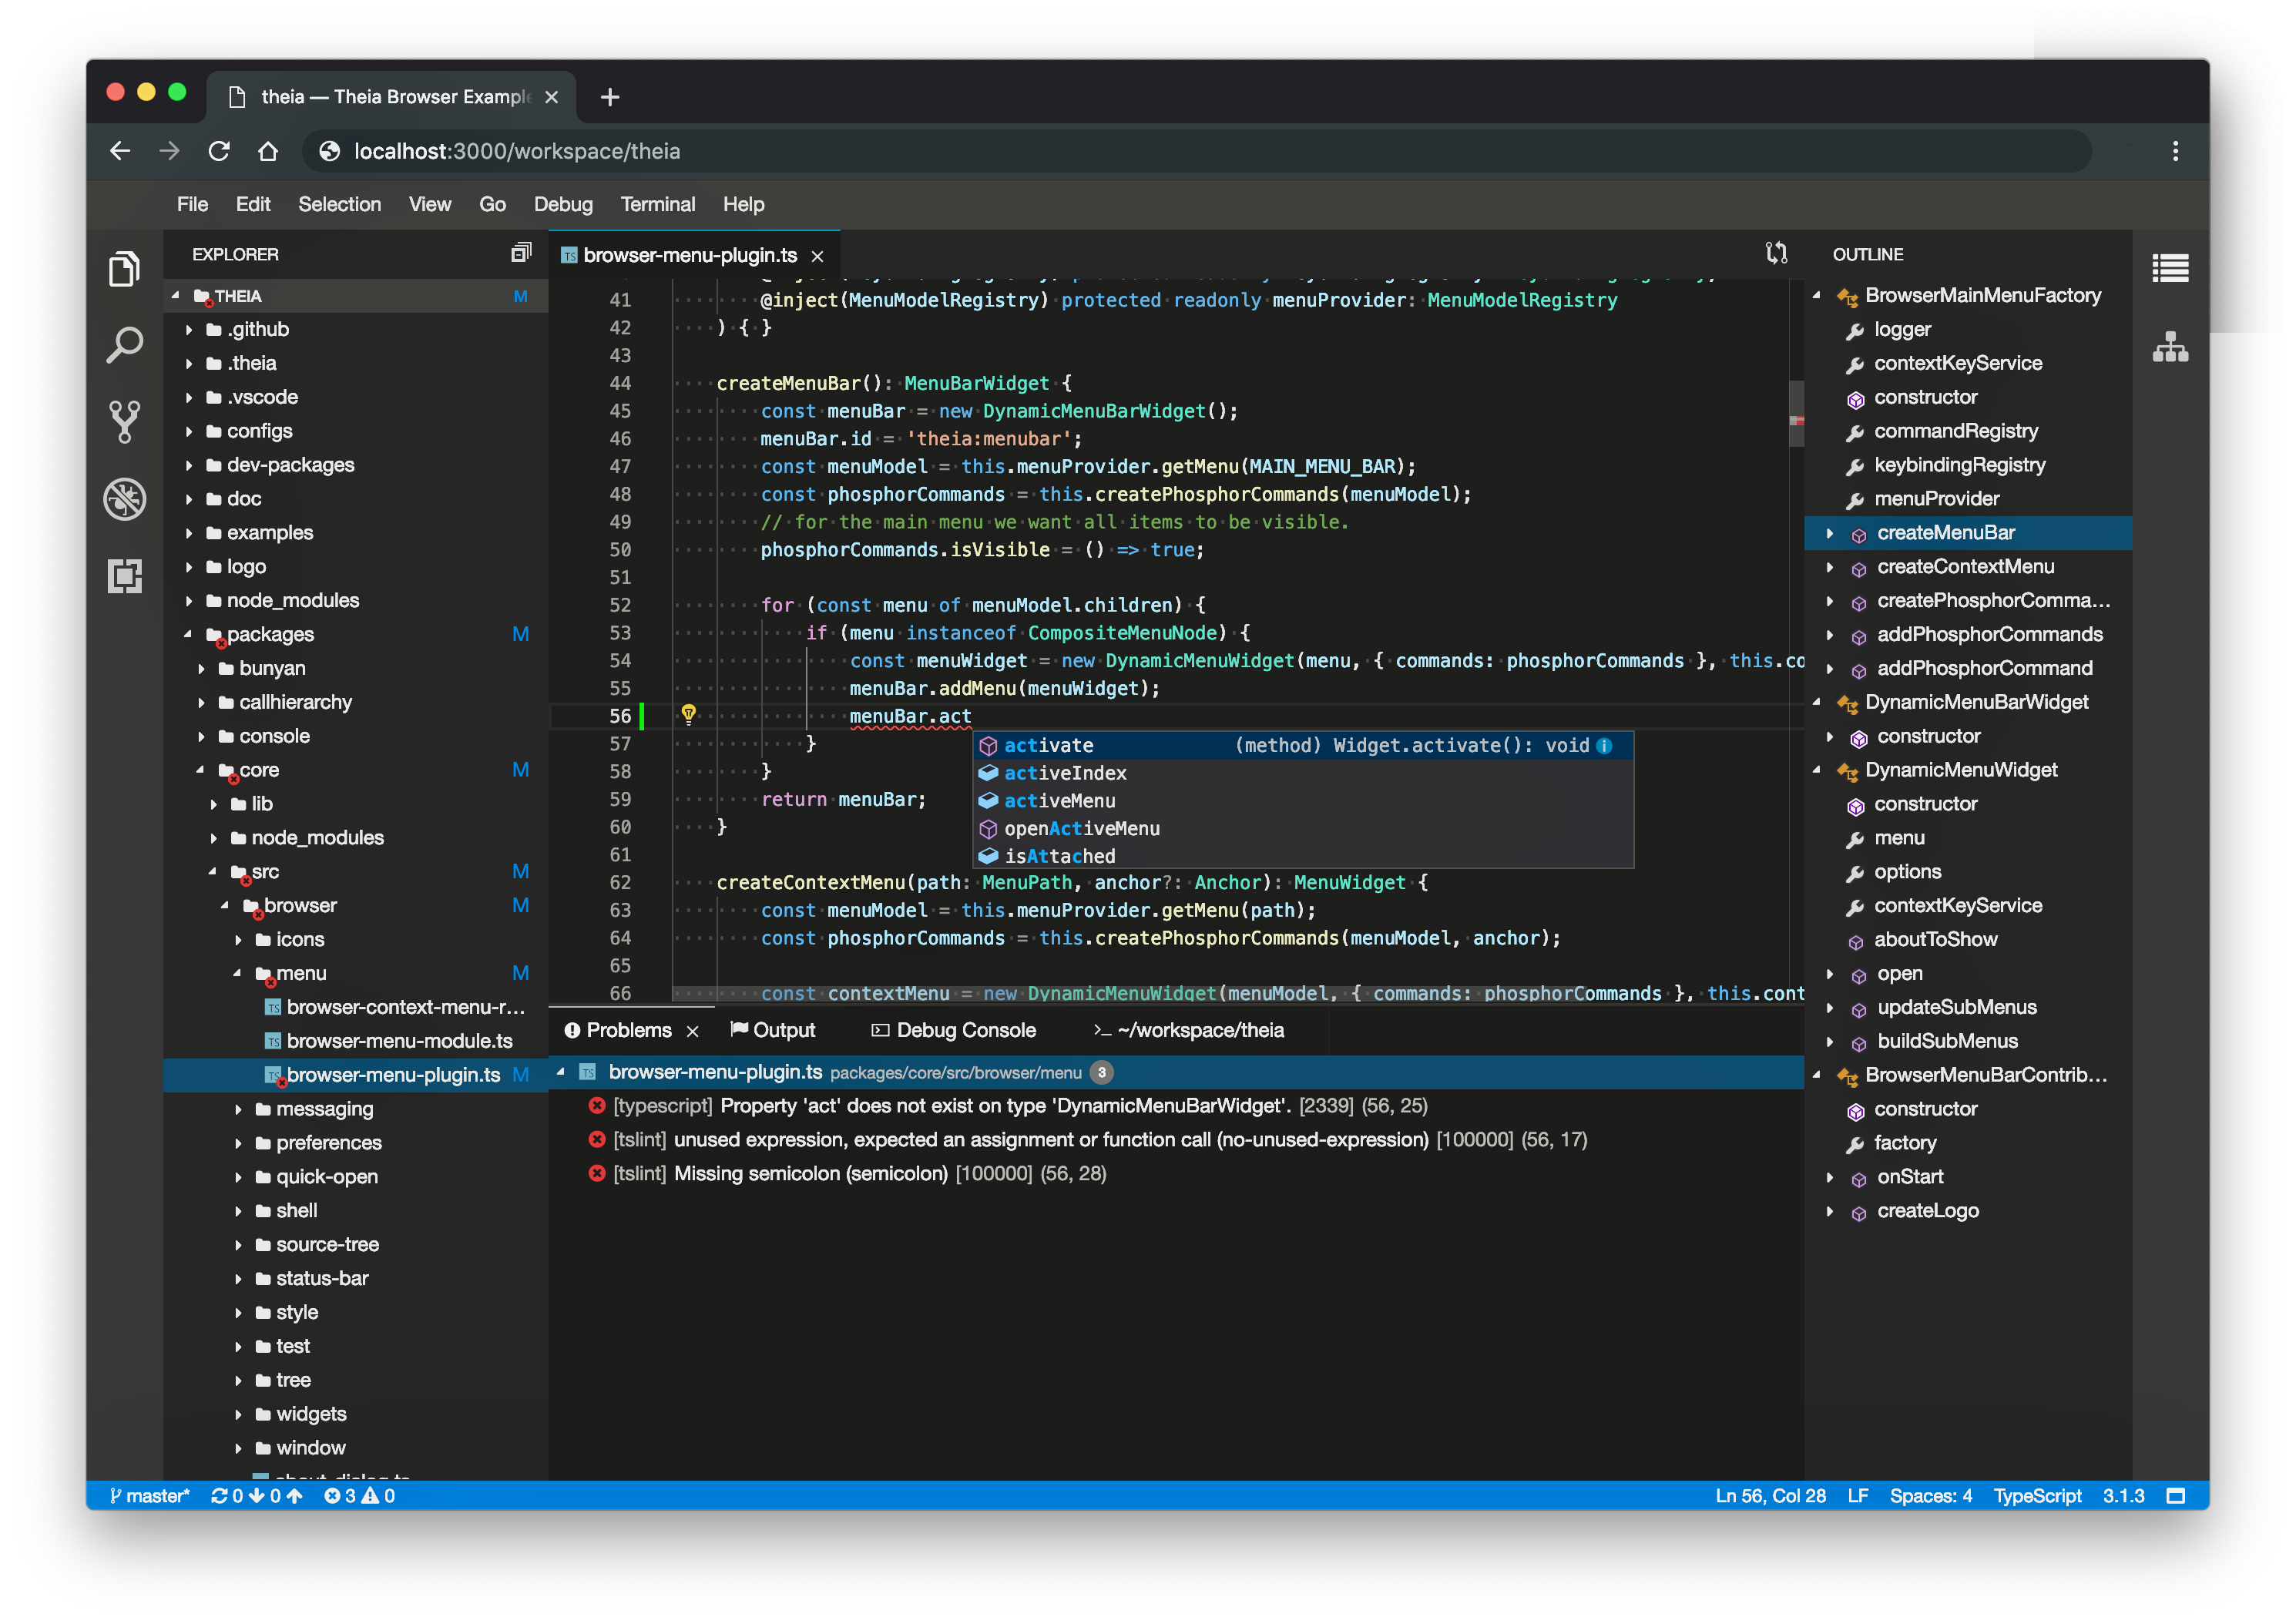
\includegraphics[width=\textwidth]{figures/theia-screenshot.png}
  \caption[Theia User Interface]{A screenshot of the Theia user interface.~\cite{eclipsefoundationEclipsetheiaTheia2020}}\label{fig:theia-user-interface}
\end{figure}

\paragraph*{Intended use}
\Gls{Theia} was created to be a framework for creating custom and
white-labeled \acrshortpl{IDE} and tools. Theia itself was not an IDE.~\cite{helmingEclipseTheiaIDE2019}

\paragraph*{Architecture --- runtime}
The architecture of Theia is similar to \gls{VSCode}.
The biggest difference is in the runtime.
\Gls{Theia} is split into a backend and frontend process. 
The backend \textit{could} run remotely, or locally. 
The frontend is \gls{Electron} or a browser.
The backend and frontend communicate with \gls{JSON-RPC} over \glspl{WebSocket} or \gls{REST}/HTTP\@. 
Both the frontend and backend source codes are heavily architected around
\emph{dependency injection}.
The backend runs an \texttt{ExpressJs} web server which serves code to the frontend (see \cref{fig:theia-communication}).~\cite{typefoxArchitectureOverview}

The frontend can always assume it has \texttt{browser API}, but not
\texttt{NodeJS}/\texttt{Electron} \gls{API}.~\cite{typefoxArchitectureOverview}

To support different programming languages, the backend talks over the \acrfull{LSP} with different \emph{language servers}.
One backend process serves one workspace/user.
Multiple clients can connect, but they will all share the same workspace.~\cite{MultiLanguageIDEImplemented2017}

\begin{figure}[htbp]
  \centering
  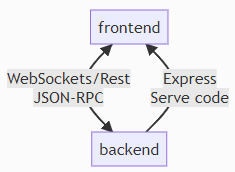
\includegraphics[width=4cm]{figures/theia-api.png}
  \caption[Theia frontend and backend communication]{Theia serves the frontend with ExpressJs and communicates between the frontend and backend with JSON-RPC.}\label{fig:theia-communication}
\end{figure}

\paragraph*{Architecture --- components}
\Gls{Theia} uses a extension oriented design.
This means that almost all functionality is provided as a \emph{Theia Extension} (see \cref{sec:theia-extension}).
For example, the \acrshortpl{API} for user-installable \emph{Theia Plugins} (see \cref{sec:theia-plugin}) are provided as an extension.
The \emph{Monaco} editor from \gls{VSCode} is also provided by an extension.
The main components of Theia is shown in \cref{fig:theia-components}.
(Note that this diagram is from 2017 and could be outdated).
The components are separated into frontend, backend and external (blue).
External resources could be processes for language compilation, package managers, terminal shells etc..

Of particular interest is the \texttt{Extensions} component with \texttt{Inversify.js}. This is the dependency injection mechanism which loads other extensions into Theia. (Also note that the \texttt{Plugin} extension for \gls{VSCode} extensions is missing in this diagram. That component was added later by RedHat\footnote{RedHat chose to use Theia in \gls{Che}, and wanted plugins that could be installed by users during run-time. They opted for the \gls{VSCode} extension mechanism for this.}.)

\begin{figure}[htbp]  % order of priority: h here, t top, b bottom, p page
  \centering
  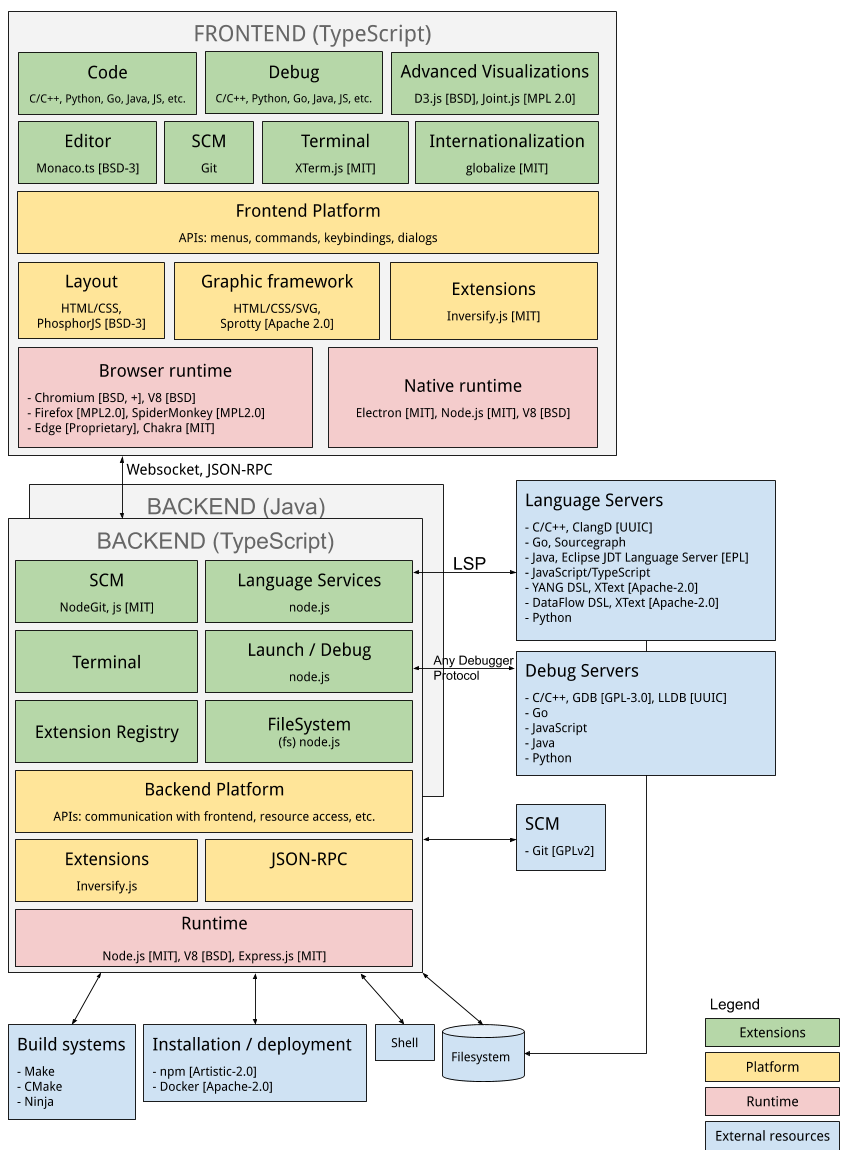
\includegraphics[width=\textwidth]{figures/Multi-Language-IDE-implemented-in-JS-Scope-and-Architecture}
  \caption[Theia module Architecture]{The main components in Theia. Some components have third party libraries, languages or runtimes listed under their component name, as examples. The figure is from a design document made in 2017, and could be outdated. (The author is unknown, but assumed to be a TypeFox employee. The document is linked to on the official Theia website).~\cite{MultiLanguageIDEImplemented2017}}\label{fig:theia-components}
\end{figure}

\paragraph*{Architecture --- code organization}
Every extension in Theia is organized based on the runtime dependencies.
This is similar to how \gls{VSCode} does it.
See \cref{fig:theia-organization}. The main difference is \texttt{electron-sandbox} in \gls{VSCode} and \texttt{electron-main} in Theia.
Every Theia extension can also provide two entrypoints: \texttt{frontend} and \texttt{backend}. This allows extensions to provide different code for the different parts of Theia. %TODO: Add cref to theia extensions

\begin{figure}[htbp]  % order of priority: h here, t top, b bottom, p page
  \centering
  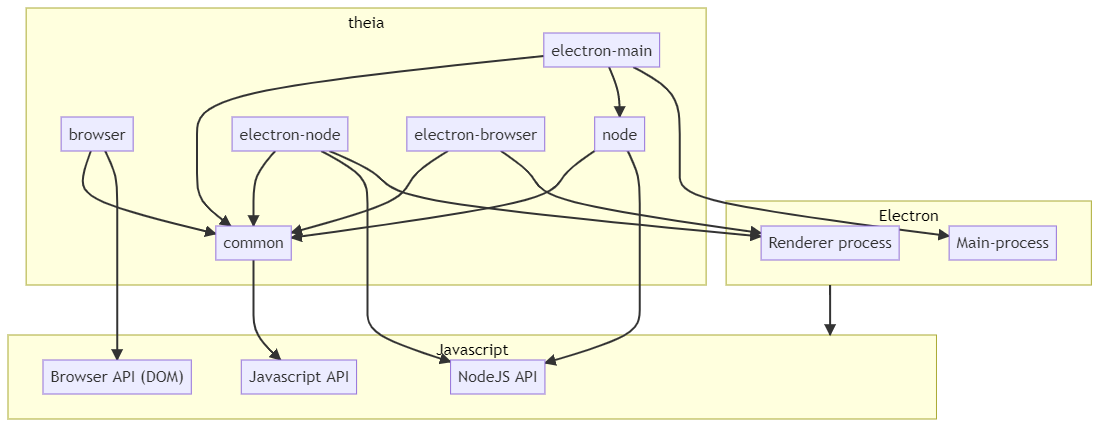
\includegraphics[width=\textwidth]{figures/theia-code-organization}
  \caption[Theia code organization]{The code in Theia extensions are organized based on the dependency on runtime \acrshortpl{API}. The box named \texttt{theia} represents an extension in Theia.~\cite{antonkosyakovCodeOrganization2019}}\label{fig:theia-organization}
\end{figure}

% What does it do?
% Who made it?
% Architecture

\subsubsection{Eclipse IDE}\label{sec:eclipse-ide}
% What does it do?
% Who made it?
% Architecture

\paragraph*{What it is}
%TODO: write

\paragraph*{Intended use}

\paragraph*{Architecture}

